\documentclass{article}\usepackage[]{graphicx}\usepackage[]{color}
%% maxwidth is the original width if it is less than linewidth
%% otherwise use linewidth (to make sure the graphics do not exceed the margin)
\makeatletter
\def\maxwidth{ %
  \ifdim\Gin@nat@width>\linewidth
    \linewidth
  \else
    \Gin@nat@width
  \fi
}
\makeatother

\definecolor{fgcolor}{rgb}{0.345, 0.345, 0.345}
\newcommand{\hlnum}[1]{\textcolor[rgb]{0.686,0.059,0.569}{#1}}%
\newcommand{\hlstr}[1]{\textcolor[rgb]{0.192,0.494,0.8}{#1}}%
\newcommand{\hlcom}[1]{\textcolor[rgb]{0.678,0.584,0.686}{\textit{#1}}}%
\newcommand{\hlopt}[1]{\textcolor[rgb]{0,0,0}{#1}}%
\newcommand{\hlstd}[1]{\textcolor[rgb]{0.345,0.345,0.345}{#1}}%
\newcommand{\hlkwa}[1]{\textcolor[rgb]{0.161,0.373,0.58}{\textbf{#1}}}%
\newcommand{\hlkwb}[1]{\textcolor[rgb]{0.69,0.353,0.396}{#1}}%
\newcommand{\hlkwc}[1]{\textcolor[rgb]{0.333,0.667,0.333}{#1}}%
\newcommand{\hlkwd}[1]{\textcolor[rgb]{0.737,0.353,0.396}{\textbf{#1}}}%

\usepackage{framed}
\makeatletter
\newenvironment{kframe}{%
 \def\at@end@of@kframe{}%
 \ifinner\ifhmode%
  \def\at@end@of@kframe{\end{minipage}}%
  \begin{minipage}{\columnwidth}%
 \fi\fi%
 \def\FrameCommand##1{\hskip\@totalleftmargin \hskip-\fboxsep
 \colorbox{shadecolor}{##1}\hskip-\fboxsep
     % There is no \\@totalrightmargin, so:
     \hskip-\linewidth \hskip-\@totalleftmargin \hskip\columnwidth}%
 \MakeFramed {\advance\hsize-\width
   \@totalleftmargin\z@ \linewidth\hsize
   \@setminipage}}%
 {\par\unskip\endMakeFramed%
 \at@end@of@kframe}
\makeatother

\definecolor{shadecolor}{rgb}{.97, .97, .97}
\definecolor{messagecolor}{rgb}{0, 0, 0}
\definecolor{warningcolor}{rgb}{1, 0, 1}
\definecolor{errorcolor}{rgb}{1, 0, 0}
\newenvironment{knitrout}{}{} % an empty environment to be redefined in TeX

\usepackage{alltt}
\usepackage[sc]{mathpazo}
\usepackage[T1]{fontenc}
\usepackage{geometry}
\geometry{verbose,tmargin=2.5cm,bmargin=2.5cm,lmargin=2.5cm,rmargin=2.5cm}
\setcounter{secnumdepth}{2}
\setcounter{tocdepth}{2}
\usepackage{url}
\usepackage[unicode=true,pdfusetitle,
 bookmarks=true,bookmarksnumbered=true,bookmarksopen=true,bookmarksopenlevel=2,
 breaklinks=false,pdfborder={0 0 1},backref=false,colorlinks=false]
 {hyperref}
\hypersetup{
 pdfstartview={XYZ null null 1}}
\usepackage{breakurl}
\IfFileExists{upquote.sty}{\usepackage{upquote}}{}
\begin{document}



\section*{Problem 4}
\begin{knitrout}
\definecolor{shadecolor}{rgb}{0.969, 0.969, 0.969}\color{fgcolor}\begin{kframe}
\begin{alltt}
\hlkwd{library}\hlstd{(MASS)}
\hlkwd{set.seed}\hlstd{(}\hlnum{20}\hlstd{)}
\hlstd{X} \hlkwb{<-} \hlkwd{data.frame}\hlstd{(}\hlkwd{rnorm}\hlstd{(}\hlnum{100}\hlstd{),} \hlkwd{rnorm}\hlstd{(}\hlnum{100}\hlstd{),} \hlkwd{rnorm}\hlstd{(}\hlnum{100}\hlstd{),} \hlkwd{rnorm}\hlstd{(}\hlnum{100}\hlstd{),} \hlkwd{rnorm}\hlstd{(}\hlnum{100}\hlstd{),}
    \hlkwd{rnorm}\hlstd{(}\hlnum{100}\hlstd{),} \hlkwd{rnorm}\hlstd{(}\hlnum{100}\hlstd{))}
\hlstd{prin_X} \hlkwb{<-} \hlkwd{prcomp}\hlstd{(X)}
\hlkwd{screeplot}\hlstd{(prin_X,} \hlkwc{main} \hlstd{=} \hlstr{"Bad ScreePlot"}\hlstd{)}
\end{alltt}
\end{kframe}

{\centering 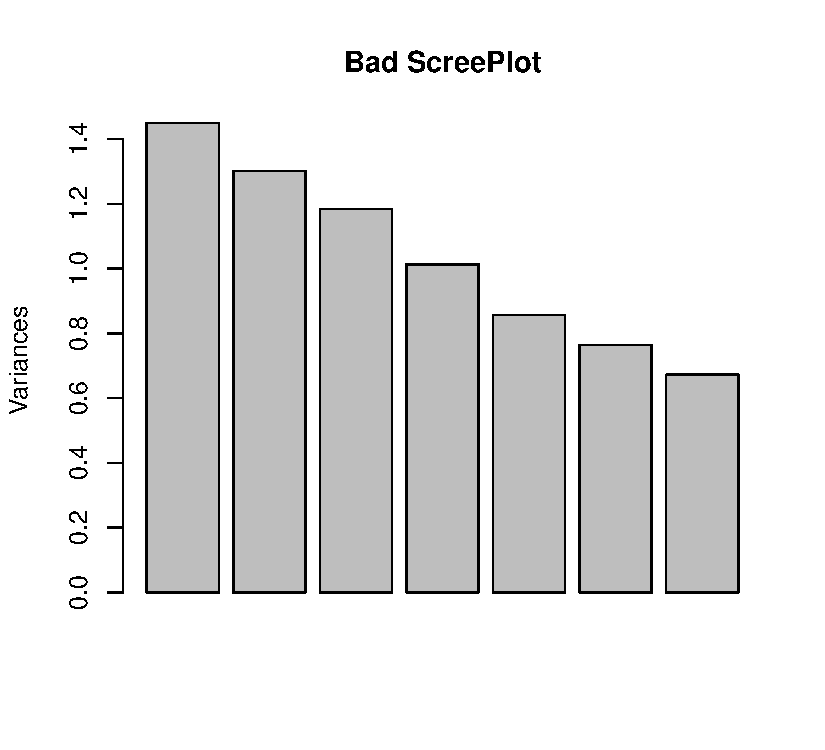
\includegraphics[width=\maxwidth]{figure/minimal-Problem_41} 

}


\begin{kframe}\begin{alltt}
\hlcom{# Comment: This is a bad screeplot since all of the principla components}
\hlcom{# have similar variance. Thus, we can not use some of the principal}
\hlcom{# compents to compress the data through projection.We need to use all of}
\hlcom{# the principal components since each of them contain similar amount of}
\hlcom{# information.}
\hlstd{Y} \hlkwb{<-} \hlkwd{data.frame}\hlstd{(}\hlkwd{rnorm}\hlstd{(}\hlnum{100}\hlstd{),} \hlkwd{rnorm}\hlstd{(}\hlnum{100}\hlstd{),} \hlkwd{rnorm}\hlstd{(}\hlnum{100}\hlstd{),} \hlkwd{rnorm}\hlstd{(}\hlnum{100}\hlstd{),} \hlkwd{rnorm}\hlstd{(}\hlnum{100}\hlstd{),}
    \hlkwd{rnorm}\hlstd{(}\hlnum{100}\hlstd{),} \hlkwd{rnorm}\hlstd{(}\hlnum{100}\hlstd{,} \hlkwc{sd} \hlstd{=} \hlnum{10}\hlstd{))}
\hlstd{prin_Y} \hlkwb{<-} \hlkwd{prcomp}\hlstd{(Y)}
\hlkwd{screeplot}\hlstd{(prin_Y,} \hlkwc{main} \hlstd{=} \hlstr{"Good ScreePlot"}\hlstd{)}
\end{alltt}
\end{kframe}

{\centering 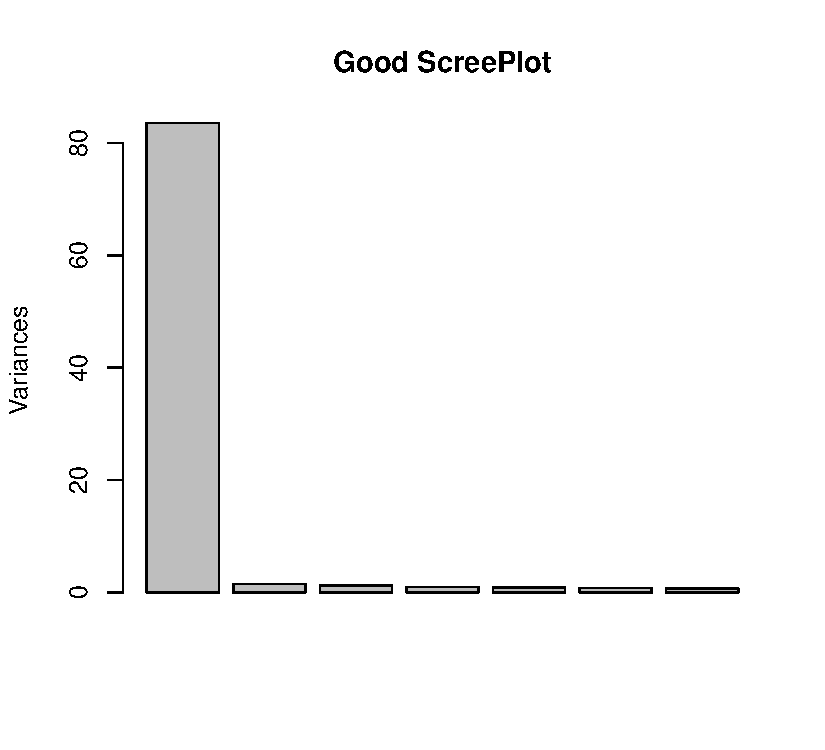
\includegraphics[width=\maxwidth]{figure/minimal-Problem_42} 

}


\begin{kframe}\begin{alltt}
# Comment: This is a good screeplot since the first principal component
# containa a large amount of information. We can use it to compress data
# and project point based on first principal component.
\end{alltt}
\end{kframe}
\end{knitrout}


\section*{Problem 5}
\begin{knitrout}
\definecolor{shadecolor}{rgb}{0.969, 0.969, 0.969}\color{fgcolor}\begin{kframe}
\begin{alltt}
\hlkwd{set.seed}\hlstd{(}\hlnum{250}\hlstd{)}
\hlstd{simulation} \hlkwb{<-} \hlkwd{cbind}\hlstd{(}\hlkwd{matrix}\hlstd{(}\hlkwd{rnorm}\hlstd{(}\hlnum{1000}\hlstd{),} \hlkwc{nrow} \hlstd{=} \hlnum{100}\hlstd{),} \hlkwd{matrix}\hlstd{(}\hlkwd{rnorm}\hlstd{(}\hlnum{300}\hlstd{,} \hlkwc{sd} \hlstd{=} \hlnum{2.5}\hlstd{),}
    \hlkwc{nrow} \hlstd{=} \hlnum{100}\hlstd{))}
\hlkwd{screeplot}\hlstd{(}\hlkwd{prcomp}\hlstd{(simulation),} \hlkwc{main} \hlstd{=} \hlstr{"dimension 100 * 13"}\hlstd{,} \hlkwc{ylim} \hlstd{=} \hlkwd{c}\hlstd{(}\hlnum{0}\hlstd{,} \hlnum{10}\hlstd{))}
\end{alltt}
\end{kframe}

{\centering 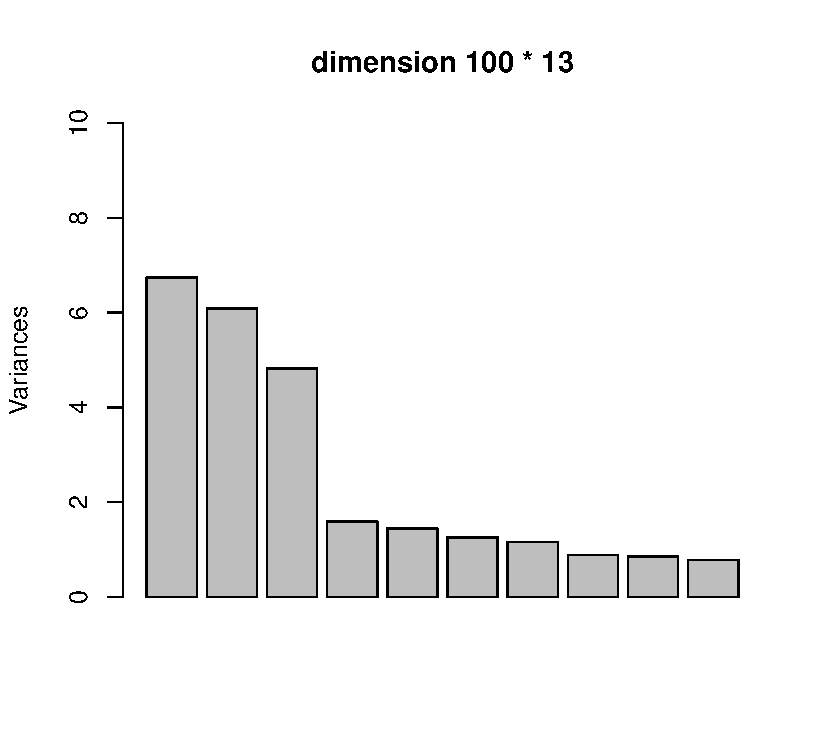
\includegraphics[width=\maxwidth]{figure/minimal-Problem_51} 

}


\begin{kframe}\begin{alltt}
\hlstd{simulation_1} \hlkwb{<-} \hlkwd{cbind}\hlstd{(}\hlkwd{matrix}\hlstd{(}\hlkwd{rnorm}\hlstd{(}\hlnum{2000}\hlstd{),} \hlkwc{nrow} \hlstd{=} \hlnum{100}\hlstd{),} \hlkwd{matrix}\hlstd{(}\hlkwd{rnorm}\hlstd{(}\hlnum{300}\hlstd{,}
    \hlkwc{sd} \hlstd{=} \hlnum{2.5}\hlstd{),} \hlkwc{nrow} \hlstd{=} \hlnum{100}\hlstd{))}
\hlkwd{screeplot}\hlstd{(}\hlkwd{prcomp}\hlstd{(simulation_1),} \hlkwc{main} \hlstd{=} \hlstr{"dimension 100 * 23"}\hlstd{,} \hlkwc{ylim} \hlstd{=} \hlkwd{c}\hlstd{(}\hlnum{0}\hlstd{,}
    \hlnum{10}\hlstd{))}
\end{alltt}
\end{kframe}

{\centering 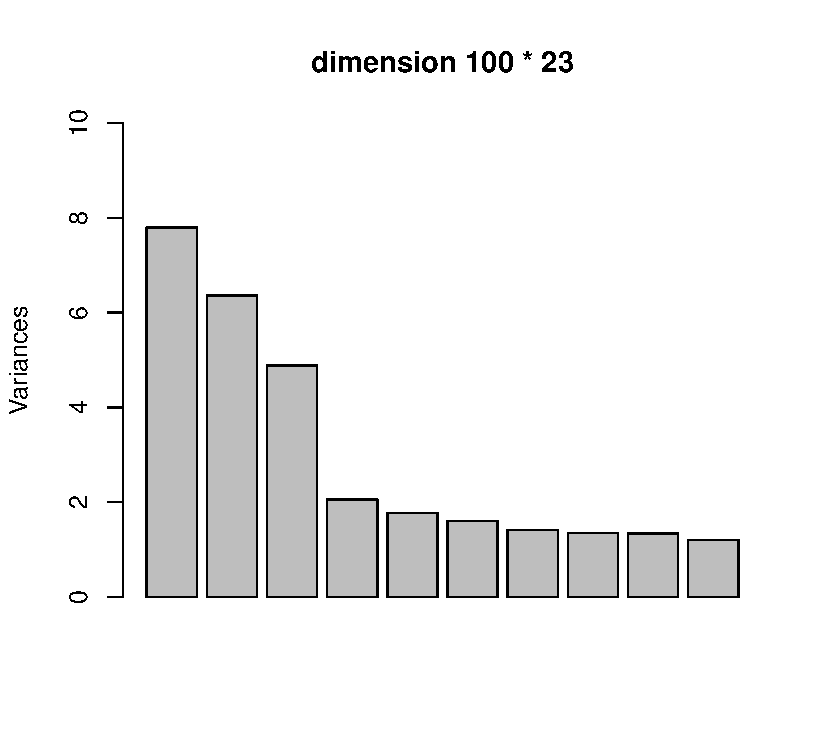
\includegraphics[width=\maxwidth]{figure/minimal-Problem_52} 

}


\begin{kframe}\begin{alltt}
\hlstd{simulation_2} \hlkwb{<-} \hlkwd{cbind}\hlstd{(}\hlkwd{matrix}\hlstd{(}\hlkwd{rnorm}\hlstd{(}\hlnum{4000}\hlstd{),} \hlkwc{nrow} \hlstd{=} \hlnum{100}\hlstd{),} \hlkwd{matrix}\hlstd{(}\hlkwd{rnorm}\hlstd{(}\hlnum{300}\hlstd{,}
    \hlkwc{sd} \hlstd{=} \hlnum{2.5}\hlstd{),} \hlkwc{nrow} \hlstd{=} \hlnum{100}\hlstd{))}
\hlkwd{screeplot}\hlstd{(}\hlkwd{prcomp}\hlstd{(simulation_1),} \hlkwc{main} \hlstd{=} \hlstr{"dimension 100 * 43"}\hlstd{,} \hlkwc{ylim} \hlstd{=} \hlkwd{c}\hlstd{(}\hlnum{0}\hlstd{,}
    \hlnum{10}\hlstd{))}
\end{alltt}
\end{kframe}

{\centering 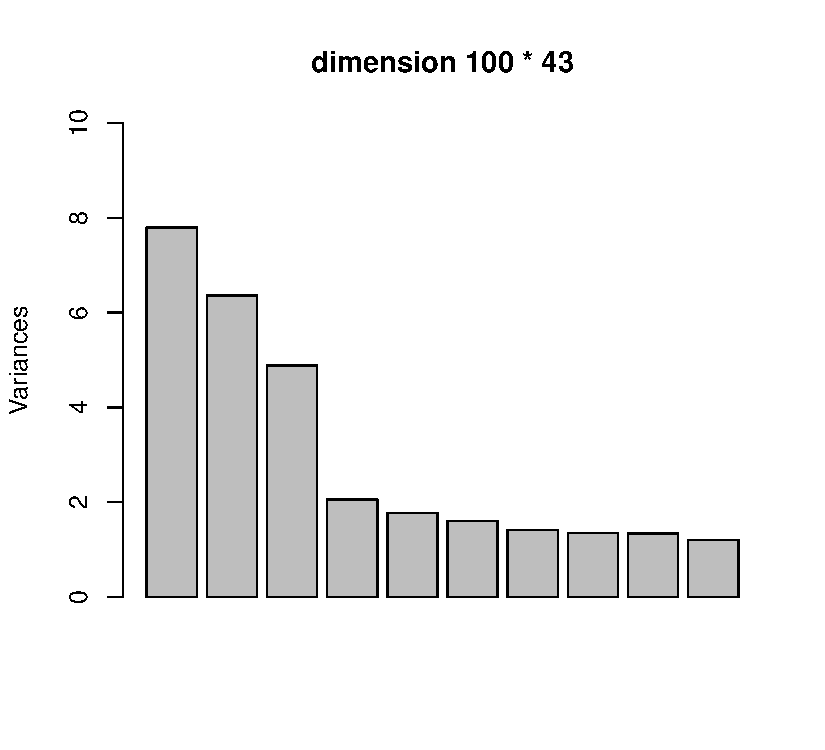
\includegraphics[width=\maxwidth]{figure/minimal-Problem_53} 

}


\begin{kframe}\begin{alltt}
\hlstd{simulation_3} \hlkwb{<-} \hlkwd{cbind}\hlstd{(}\hlkwd{matrix}\hlstd{(}\hlkwd{rnorm}\hlstd{(}\hlnum{5000}\hlstd{),} \hlkwc{nrow} \hlstd{=} \hlnum{100}\hlstd{),} \hlkwd{matrix}\hlstd{(}\hlkwd{rnorm}\hlstd{(}\hlnum{300}\hlstd{,}
    \hlkwc{sd} \hlstd{=} \hlnum{2.5}\hlstd{),} \hlkwc{nrow} \hlstd{=} \hlnum{100}\hlstd{))}
\hlkwd{screeplot}\hlstd{(}\hlkwd{prcomp}\hlstd{(simulation_3),} \hlkwc{main} \hlstd{=} \hlstr{"dimension 100 * 53"}\hlstd{,} \hlkwc{ylim} \hlstd{=} \hlkwd{c}\hlstd{(}\hlnum{0}\hlstd{,}
    \hlnum{10}\hlstd{))}
\end{alltt}
\end{kframe}

{\centering 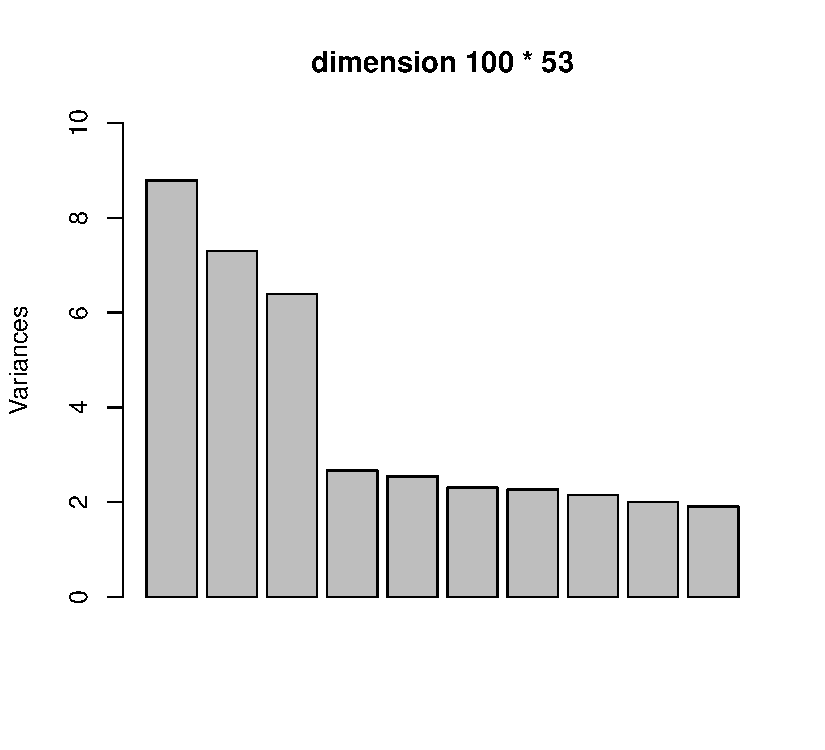
\includegraphics[width=\maxwidth]{figure/minimal-Problem_54} 

}


\begin{kframe}\begin{alltt}
\hlstd{simulation_4} \hlkwb{<-} \hlkwd{cbind}\hlstd{(}\hlkwd{matrix}\hlstd{(}\hlkwd{rnorm}\hlstd{(}\hlnum{10000}\hlstd{),} \hlkwc{nrow} \hlstd{=} \hlnum{100}\hlstd{),} \hlkwd{matrix}\hlstd{(}\hlkwd{rnorm}\hlstd{(}\hlnum{300}\hlstd{,}
    \hlkwc{sd} \hlstd{=} \hlnum{2.5}\hlstd{),} \hlkwc{nrow} \hlstd{=} \hlnum{100}\hlstd{))}
\hlkwd{screeplot}\hlstd{(}\hlkwd{prcomp}\hlstd{(simulation_4),} \hlkwc{main} \hlstd{=} \hlstr{"dimension 100 * 103"}\hlstd{,} \hlkwc{ylim} \hlstd{=} \hlkwd{c}\hlstd{(}\hlnum{0}\hlstd{,}
    \hlnum{10}\hlstd{))}
\end{alltt}
\end{kframe}

{\centering 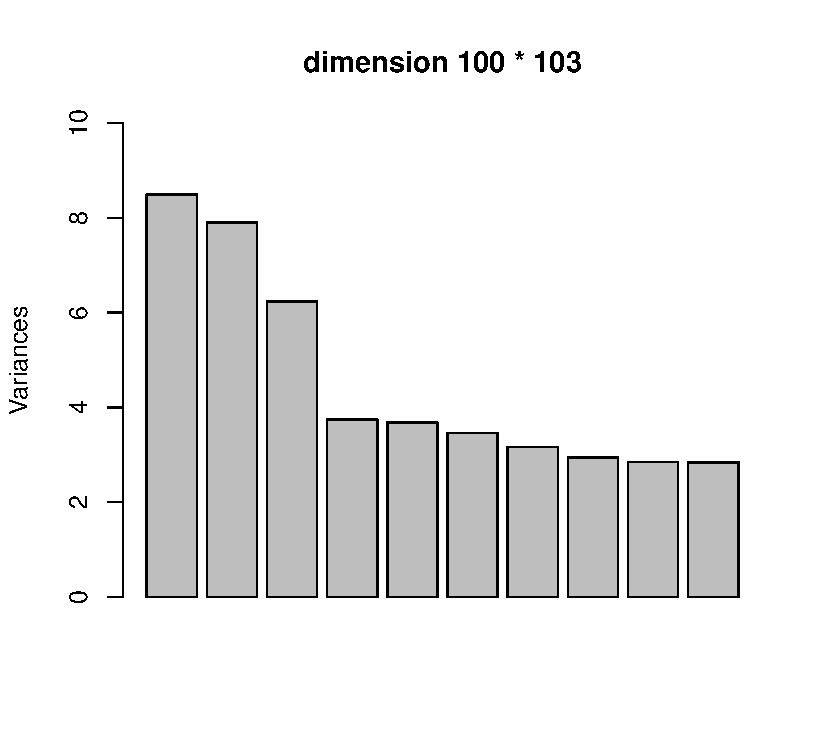
\includegraphics[width=\maxwidth]{figure/minimal-Problem_55} 

}


\begin{kframe}\begin{alltt}
\hlstd{simulation_5} \hlkwb{<-} \hlkwd{cbind}\hlstd{(}\hlkwd{matrix}\hlstd{(}\hlkwd{rnorm}\hlstd{(}\hlnum{20000}\hlstd{),} \hlkwc{nrow} \hlstd{=} \hlnum{100}\hlstd{),} \hlkwd{matrix}\hlstd{(}\hlkwd{rnorm}\hlstd{(}\hlnum{300}\hlstd{,}
    \hlkwc{sd} \hlstd{=} \hlnum{2.5}\hlstd{),} \hlkwc{nrow} \hlstd{=} \hlnum{100}\hlstd{))}
\hlkwd{screeplot}\hlstd{(}\hlkwd{prcomp}\hlstd{(simulation_5),} \hlkwc{main} \hlstd{=} \hlstr{"dimension 100 * 203"}\hlstd{,} \hlkwc{ylim} \hlstd{=} \hlkwd{c}\hlstd{(}\hlnum{0}\hlstd{,}
    \hlnum{10}\hlstd{))}
\end{alltt}
\end{kframe}

{\centering 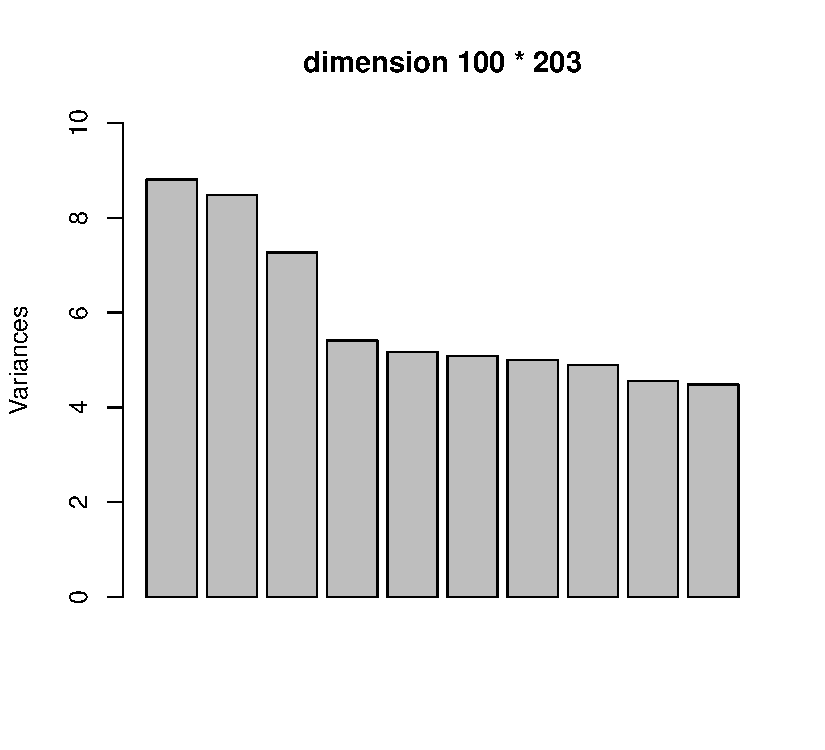
\includegraphics[width=\maxwidth]{figure/minimal-Problem_56} 

}



\end{knitrout}

Comment: The matrix is constructed so that there are three columns with obvious variability and the other columns have less variability. So we will expect to have three principal components contributing more variability. However, as we increase the number of columns with less varied data, it turns out that the screeplot will explain less variability, which means that increasing dimension would make the variability more ambient data less interpretable using PCA.

\section*{Problem 6}
\begin{knitrout}
\definecolor{shadecolor}{rgb}{0.969, 0.969, 0.969}\color{fgcolor}\begin{kframe}
\begin{alltt}
\hlkwd{set.seed}\hlstd{(}\hlnum{100}\hlstd{)}
\hlstd{A} \hlkwb{<-} \hlkwd{matrix}\hlstd{(}\hlnum{0}\hlstd{,} \hlkwc{nrow} \hlstd{=} \hlnum{20}\hlstd{,} \hlkwc{ncol} \hlstd{=} \hlnum{20}\hlstd{)}
\hlstd{eigenvalue} \hlkwb{<-} \hlkwd{c}\hlstd{(}\hlnum{4}\hlstd{,} \hlnum{4}\hlstd{,} \hlnum{4}\hlstd{,} \hlnum{4}\hlstd{,} \hlkwd{rep}\hlstd{(}\hlnum{1.025}\hlstd{,} \hlnum{16}\hlstd{))}
\hlkwd{diag}\hlstd{(A)} \hlkwb{<-} \hlstd{eigenvalue}
\hlcom{# Now we need to construct an orthogonal matrix, I did this by doing svd}
\hlcom{# decomposition to a 8x8 random matrix a extract the U matrix.}
\hlstd{f} \hlkwb{<-} \hlkwa{function}\hlstd{() \{}
    \hlstd{U} \hlkwb{<-} \hlkwd{svd}\hlstd{(}\hlkwd{matrix}\hlstd{(}\hlkwd{rnorm}\hlstd{(}\hlnum{400}\hlstd{),} \hlnum{20}\hlstd{))}\hlopt{$}\hlstd{u}
    \hlcom{# Then I can construct a Z matrix}
    \hlstd{Z} \hlkwb{<-} \hlstd{U} \hlopt \hlstd{A} \hlopt \hlkwd{t}\hlstd{(U)}
    \hlstd{prin_Z} \hlkwb{<-} \hlkwd{prcomp}\hlstd{(Z)}
    \hlstd{explain_var_Z} \hlkwb{<-} \hlkwd{sapply}\hlstd{(}\hlnum{1}\hlopt{:}\hlnum{20}\hlstd{,} \hlkwa{function}\hlstd{(}\hlkwc{i}\hlstd{)} \hlkwd{sum}\hlstd{(prin_Z}\hlopt{$}\hlstd{sdev[}\hlnum{1}\hlopt{:}\hlstd{i]}\hlopt{^}\hlnum{2}\hlstd{)}\hlopt{/}\hlkwd{sum}\hlstd{(prin_Z}\hlopt{$}\hlstd{sdev}\hlopt{^}\hlnum{2}\hlstd{))}
    \hlkwd{return}\hlstd{(}\hlkwd{head}\hlstd{(explain_var_Z,} \hlnum{4}\hlstd{))}
\hlstd{\}}
\hlstd{Rep} \hlkwb{<-} \hlkwd{replicate}\hlstd{(}\hlnum{2000}\hlstd{,} \hlkwd{f}\hlstd{())}
\hlkwd{rowMeans}\hlstd{(Rep)}
\end{alltt}
\begin{verbatim}
## [1] 0.2085 0.4171 0.6256 0.7946
\end{verbatim}
\begin{alltt}
\hlkwd{hist}\hlstd{(Rep[}\hlnum{1}\hlstd{, ],} \hlkwc{breaks} \hlstd{=} \hlkwd{seq}\hlstd{(}\hlnum{0.2}\hlstd{,} \hlnum{0.24}\hlstd{,} \hlkwc{by} \hlstd{=} \hlnum{5e-04}\hlstd{),} \hlkwc{main} \hlstd{=} \hlstr{"Percent of Explained Variance of the First PC"}\hlstd{,}
    \hlkwc{xlab} \hlstd{=} \hlstr{"PC_1"}\hlstd{)}
\end{alltt}
\end{kframe}

{\centering 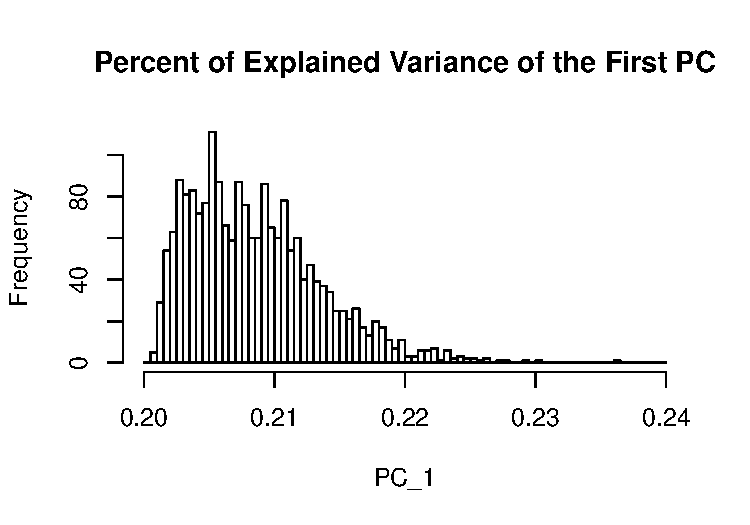
\includegraphics[width=\maxwidth]{figure/minimal-Problem_61} 

}


\begin{kframe}\begin{alltt}
\hlkwd{hist}\hlstd{(Rep[}\hlnum{4}\hlstd{, ],} \hlkwc{breaks} \hlstd{=} \hlkwd{seq}\hlstd{(}\hlnum{0.765}\hlstd{,} \hlnum{0.81}\hlstd{,} \hlkwc{by} \hlstd{=} \hlnum{5e-04}\hlstd{),} \hlkwc{main} \hlstd{=} \hlstr{"Percent of Explained Variance of the First Four PCs"}\hlstd{,}
    \hlkwc{xlab} \hlstd{=} \hlstr{"First 4 PCs"}\hlstd{)}
\end{alltt}
\end{kframe}

{\centering 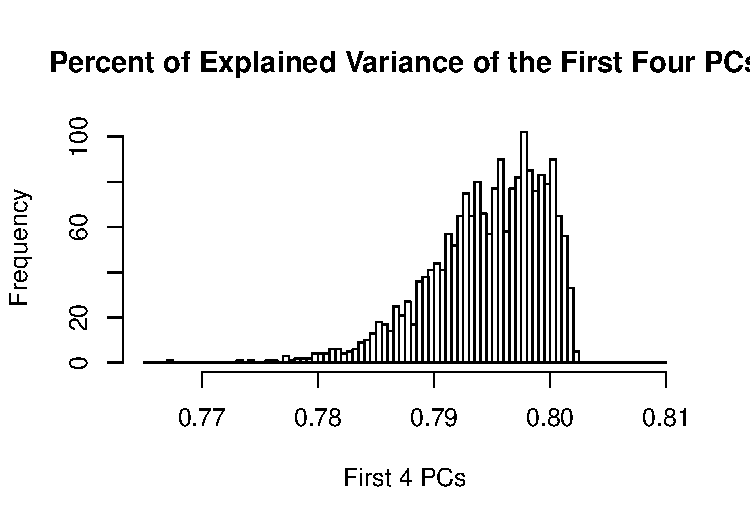
\includegraphics[width=\maxwidth]{figure/minimal-Problem_62} 

}



\end{knitrout}

Comment: I did this problem by constructing a diagnal matrix A with first four diagnal elements as 2 and the rest are smaller, then pretend it is the eigen matrix of some decomposed matrix using svd. Then, I construct the "original" matrix by multiplying orthogonal matrix to A. The method is the same as doing SVD decomposition backwards. Then, I replicate the function 2000 times to get the average of the explanation first four PCs. By the output, we have four three eigen vector explaining raughly 20 percent variability each, and the rest explain 20 percent variability.\\
        In terms of stability; by first histogram, it seems that the the first principal component tends to explain more than 20 percent of variance(heavy righ tail) although it should explain exactly the same amount of variance as the other three by construction; however, the total variance explained by the top four PCs will not exceed 80 percent but it tends to explain less than 80 percent(heavy left tail in the histogram).

\section*{Problem 7}
\begin{knitrout}
\definecolor{shadecolor}{rgb}{0.969, 0.969, 0.969}\color{fgcolor}\begin{kframe}
\begin{alltt}
\hlcom{# For N(0,1) distribution}
\hlstd{iqr} \hlkwb{<-} \hlkwd{qnorm}\hlstd{(}\hlnum{0.75}\hlstd{)} \hlopt{-} \hlkwd{qnorm}\hlstd{(}\hlnum{0.25}\hlstd{)}
\hlcom{# For N(miu, sd) distribution, IQR = sd*(qnorm(0.75) - qnorm(0.25)), I}
\hlcom{# use the following code to verify.}
\hlstd{mu} \hlkwb{<-} \hlnum{10}
\hlstd{sigma} \hlkwb{<-} \hlnum{5}
\hlstd{iqr_new} \hlkwb{<-} \hlkwd{qnorm}\hlstd{(}\hlnum{0.75}\hlstd{,} \hlkwc{mean} \hlstd{= mu,} \hlkwc{sd} \hlstd{= sigma)} \hlopt{-} \hlkwd{qnorm}\hlstd{(}\hlnum{0.25}\hlstd{,} \hlkwc{mean} \hlstd{=} \hlnum{10}\hlstd{,} \hlkwc{sd} \hlstd{= sigma)}
\hlkwd{all.equal}\hlstd{(iqr_new, sigma} \hlopt{*} \hlstd{iqr)}
\end{alltt}
\begin{verbatim}
## [1] TRUE
\end{verbatim}
\begin{alltt}
\hlcom{# For N(0,1)}
\hlstd{fraction_outlier} \hlkwb{<-} \hlnum{1} \hlopt{-} \hlkwd{pnorm}\hlstd{(}\hlkwd{qnorm}\hlstd{(}\hlnum{0.75}\hlstd{)} \hlopt{+} \hlnum{1.5} \hlopt{*} \hlstd{iqr)} \hlopt{+} \hlkwd{pnorm}\hlstd{(}\hlkwd{qnorm}\hlstd{(}\hlnum{0.25}\hlstd{)} \hlopt{-}
    \hlnum{1.5} \hlopt{*} \hlstd{iqr)}
\end{alltt}
\end{kframe}
\end{knitrout}

\subsection*{(1)}
For\emph{N}(0,1) distribution, the \emph{IQR} of is 1.349 \\
\subsection*{(2)}
For \emph{N}($\mu$,$\sigma^2$) distribution, the \emph{IQR} is going to be $\sigma$*($Q_{3}$-$Q_{1}$). In order to check it, we have use \emph{N}(10,5) to verify. It turns out its \emph{IQR} is 6.7449, which is the raughly the same as 5 *  1.349\\
\subsection*{(3)}
The fraction of outlier for \emph{N}(0,1) is roughly 0.007
\begin{quote}
\textbf{The rest of problem is attached as a hand written page}
\end{quote}


\end{document}
